Cette partie de l'application est principalement basée sur l'analyse et l'enregistrement des notes jouées par 
l'utilisateur. Le principe est d'analyser en temps réel les fréquences à la base du son de la guitare, et de faire en sort de constituer un accord
avec les notes ayant le volume le plus fort et l'enregistrer. De plus, le modèle comporte également toutes les informations sur les préférences
de l'utilisateur pour l'application,   ainsi que des fonctions pour enregistrer les données. Nous avons choisi de sauvegarder les fichiers au format JSON. \newline
Afin de jouer une partition, nous utiliserons des sons de guitare en midi d'une durée courte, que nous jouerons plusieurs fois afin de correspondre à la durée de la note sur la partition, il y aura également la possibilité de changer la note jouée pour une note qui correspond plus à sa propre guitare pour une meilleure expérience utilisateur.

\begin{figure}[H]
\centering
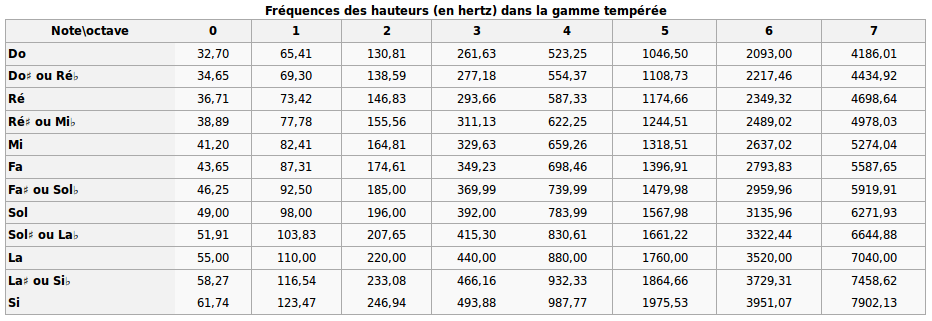
\includegraphics[scale=0.5]{Frequences}
\caption{Toutes les frequences possibles}
\end{figure}